\chapter{Návrh komponenty výukového serveru}
Třetí kapitola se primárně věnuje návrhu komponenty výukového serveru zaměřené na problematiku amortizované složitosti. Nejprve popisuje cíl a roli navrhované komponenty v rámci výukového serveru a vysvětluje její přínos pro výuku této oblasti. Následně shrnuje hlavní požadavky, které byly na komponentu kladeny, a objasňuje výběr algoritmů zařazených do praktické části práce. Další část kapitoly se zaměřuje na návrh funkcionality komponenty, zejména na způsoby zadávání vstupů, zobrazení průběhu algoritmů a prezentaci hodnot důležitých pro pochopení amortizované analýzy. Na konci kapitoly je pozornost věnována také návrhu uživatelského rozhraní, celkové struktury komponenty a možného rozšíření. 



\section{Cíl a role navrhované komponenty}
V této části je nejprve vymezeno zařazení navrhované komponenty v rámci výukového serveru. Následně je pozornost věnována hlavnímu účelu komponenty a její roli při zprostředkování problematiky amortizované složitosti studentům. V závěru této části je shrnut její přínos pro výuku a pro názornější pochopení sledované problematiky.

\newpage

\subsection{Zařazení komponenty do výukového serveru}
Vytvořená komponenta vzniká jako součást výukového serveru určeného pro předměty TI. Tento výukový server má mít podobu sady dynamických webových stránek, jejichž hlavním cílem je umožnit budoucím studentům lépe pochopit principy různých typů úloh a problémů prostřednictvím názorných a interaktivních ukázek. Na rozdíl od běžných statických výukových materiálů, které obvykle pracují pouze s pevně daným počtem příkladů, má takové řešení umožnit generovat libovolný počet ukázkových příkladů vybraných algoritmů na základě vstupů od uživatele a sledovat jejich průběh v různých situacích.

Navrhovaná komponenta je v rámci tohoto serveru zaměřena na oblast amortizované složitosti. Jejím úkolem je rozšířit výukový server o část, která studentům umožní lépe pochopit principy tohoto typu analýzy na konkrétních algoritmech a datových strukturách. Komponenta se tedy nesnaží představit samostatný izolovaný nástroj, ale stává se součástí výuky v TI a zapadá do širšího konceptu interaktivní podpory studia teoretické informatiky.

\subsection{Hlavní účel komponenty}
Hlavním účelem této navržené komponenty je vytvořit prostředek pro pochopení počítání složitosti vybraných algoritmů s využitím amortizované analýzy, která byla podrobně popsána v předchozí kapitole. Komponenta má budoucím studentům poskytnout vizualizaci toho, jak se algoritmus chová při zpracování vstupu, jak se mění stav dané datové struktury a jak probíhá vývoj hodnot v jednotlivých krocích, které jsou důležité pro amortizovanou analýzu. Důraz je kladen především na to, aby uživatel viděl podrobný průběh algoritmu v každém kroku, nikoli pouze konečný výsledek výpočtu.

Účelem komponenty tedy není pouze umožnit spuštění algoritmu, ale především podpořit hlubší pochopení celého principu, proč se amortizovaná složitost hodnotí v rámci delší posloupnosti operací. Komponenta má propojit teoretický výklad s názornou ukázkou chování algoritmu a nabídnout studentovi možnost sledovat souvislosti mezi jednotlivými operacemi a jejich dlouhodobým dopadem.

\newpage

\subsection{Přínos komponenty pro výuku amortizované složitosti}
Celá problematika amortizované složitosti bývá pro studenty často obtížně pochopitelná, protože její správné pochopení vyžaduje sledování souvislostí mezi více operacemi, změn stavů vizualizovaných datových struktur a vývoje hodnot, které se při amortizované analýze používají. Klasické výklady v teoretické formě pomocí prezentací, skript nebo několika málo statických ukázek nemusí vždy stačit k tomu, aby si studenti vytvořili dostatečně jasnou představu o tom, proč se některé operace mohou jevit jako nákladné oproti ostatním a proč je přesto možné celkové chování algoritmu hodnotit příznivěji.

Důležitý přínos této komponenty spočívá především v propojení teoretického výkladu s názornou praktickou ukázkou. Student může při práci s komponentou aktivně sledovat průběh algoritmů, pozorovat změny stavů datových struktur a lépe chápat vztah mezi jednotlivými operacemi a jejich dlouhodobým chováním. Komponenta tak může přispět k názornější a srozumitelnější výuce amortizované složitosti v rámci předmětů TI.



\section{Požadavky na komponentu}
Tato část se zaměřuje na hlavní požadavky, které byly na navrhovanou komponentu kladeny. Nejprve jsou shrnuty funkční požadavky související s chováním a možnostmi komponenty. Následně jsou popsány požadavky na uživatelskou interakci a na způsob, jakým má uživatel s komponentou pracovat. Závěr této části je věnován požadavkům na názornost a výukovou hodnotu navrhovaného řešení.

\subsection{Funkční požadavky}
Při návrhu celé komponenty bylo potřeba vycházet z požadavků, které byly stanoveny v zadání bakalářské práce. Základním funkčním požadavkem bylo vytvořit dynamické webové stránky, které umožní vhodným způsobem zobrazit simulaci běhu alespoň tří různých algoritmů, u nichž je vhodné analyzovat složitost pomocí amortizované analýzy. Komponenta tak měla uživateli umožnit nejen samotné spuštění algoritmu, ale také sledování jeho jednotlivých kroků v průběhu zpracování zadaného vstupu.

Dalším důležitým požadavkem bylo umožnit uživateli zadávat vstupy více různými způsoby. Návrh u každého algoritmu proto musel počítat s možností ručního zadávání vstupů, s generováním náhodných vstupů podle zvolených parametrů, s prací s různě velkými ukázkovými vstupy a také se zadáváním vstupů pomocí syntaxe příkazů. Komponenta měla zároveň během simulace zobrazovat informace o aktuálním stavu výpočtu, počet provedených kroků a aktuální hodnotu potenciálu nebo naspořených mincí podle použité metody amortizované analýzy. V této práci byla zvolena potenciálová metoda.

Pro lepší přehlednost shrnuje tabulka \ref{tab:functional_requirements_component} hlavní funkční požadavky navrhované komponenty.

\begin{table}[H]
\centering
\caption{Hlavní funkční požadavky navrhované komponenty}
\label{tab:functional_requirements_component}
\begin{tabular}{|p{4.2cm}|p{7.2cm}|}
\hline
\textbf{Požadavek} & \textbf{Stručný popis} \\ \hline
    Podpora více algoritmů & Komponenta musí umožnit práci alespoň se třemi algoritmy vhodnými pro amortizovanou analýzu. \\ \hline
    Různé způsoby zadávání vstupů & Uživatel musí mít možnost zadávat vstupy ručně, náhodně je generovat, pracovat s ukázkovými vstupy různé velikosti a zadávat je také pomocí syntaxe. \\ \hline
    Zobrazení průběhu algoritmu & Komponenta musí umožnit sledovat chování algoritmu v průběhu výpočtu, nikoli pouze jeho konečný výsledek. \\ \hline
    Zobrazení stavu datové struktury & V průběhu simulace musí být zobrazen aktuální stav datové struktury používané algoritmem. \\ \hline
    Zobrazení doplňujících hodnot & Součástí simulace musí být zobrazení počtu kroků a hodnot souvisejících s amortizovanou analýzou, například potenciálu nebo naspořených mincí. \\ \hline
    Podpora teoretického výkladu & Ke každému algoritmu musí být dostupné také odvození jeho složitosti jako doplnění interaktivní simulace. \\ \hline
\end{tabular}
\end{table}

Dalším funkčním požadavkem bylo také to, aby ke každému algoritmu bylo přímo v rámci vytvořené stránky, například ve formě statické části, dostupné odvození jeho složitosti. Celá komponenta podle zadání neměla sloužit pouze jako prostředek pro interaktivní simulaci, ale také jako podpora teoretického výkladu jednotlivých algoritmů a jejich amortizované analýzy.

\newpage

\subsection{Požadavky na uživatelskou interakci}
Funkčnost nebyla jedinou důležitou prioritou, ale bylo také nutné navrhnout komponentu tak, aby s ní dokázal pracovat každý uživatel přehledně a srozumitelně. Celý vzhled stránky měl působit přívětivě a zadávání vstupů mělo být navrženo tak, aby bylo přehledné a srozumitelné. Uživatel by neměl mít problém zadat libovolný vstup a v případě chyby při zadávání by měl být vhodným způsobem upozorněn na to, co zadává nesprávně.

Návrh zároveň počítal s tím, že uživatel bude moci měnit vstupy, opakovaně spouštět simulace a sledovat, jak se změny vstupu projeví v průběhu algoritmu. Důležitým požadavkem bylo také to, aby uživatel mohl snadno sledovat jednotlivé kroky výpočtu a rozuměl tomu, co se v daném okamžiku děje. Interakce s komponentou proto neměla být omezena pouze na zobrazení výsledku, ale měla podporovat průběžné vnímání změn stavu datové struktury a souvisejících hodnot.

\subsection{Požadavky na názornost a výukovou hodnotu}
Jedním z nejdůležitějších požadavků na navrhovanou komponentu byla její názornost a výuková hodnota. Nestačilo, aby komponenta technicky zobrazovala průběh algoritmu, ale bylo také nutné, aby uživateli pomáhala pochopit celou problematiku. Návrh proto musel směřovat k tomu, aby student mohl jasně sledovat vztah mezi jednotlivými operacemi, změnami stavu datové struktury a vývojem hodnot důležitých pro použitou metodu analýzy.

Výuková hodnota komponenty spočívá především v propojení teoretického výkladu s praktickou ukázkou. Uživatel nemá pouze číst popis algoritmu, ale má současně vidět jeho konkrétní chování při různých typech vstupů a lépe chápat, proč se celkové náklady algoritmu neposuzují jen podle jedné operace. Proto bylo při návrhu důležité dbát na srozumitelnost, přehlednost a na takové uspořádání informací, které podpoří lepší orientaci uživatele v průběhu simulace.



\section{Výběr algoritmů pro praktickou část}
V této části je vysvětlen výběr algoritmů zařazených do praktické části práce. Nejprve jsou uvedena hlavní kritéria, podle nichž byly algoritmy vybírány. Následně jsou představeny jednotlivé zvolené algoritmy a je objasněno, proč byly vybrány právě jako zástupci různé obtížnosti a různých projevů amortizované složitosti.

\subsection{Kritéria výběru algoritmů}
Výběr algoritmů byl velmi důležitý, protože bylo potřeba zvolit takové příklady, které budou vhodné z hlediska amortizované analýzy a současně budou přínosné pro výuku. Jedním z hlavních kritérií bylo to, že u zvolených algoritmů nebo datových struktur se mohou jednotlivé operace výrazně lišit svou skutečnou cenou, avšak při delší posloupnosti operací lze jejich chování hodnotit příznivěji pomocí amortizované analýzy.

Dalším důležitým kritériem byla rozdílná obtížnost vybraných algoritmů. Cílem bylo zařadit takové příklady, které studentům umožní postupovat od jednoduššího principu k náročnějšímu. Z tohoto důvodu byl vybrán jeden jednodušší algoritmus, jeden středně obtížný příklad a jedna pokročilejší datová struktura. Výběr byl zároveň přizpůsoben tomu, aby bylo možné jednotlivé algoritmy vhodně vizualizovat a názorně na nich ukázat různé projevy amortizované složitosti.

\subsection{Multipop na zásobníku jako jednoduchý příklad}
Jako jednodušší příklad byl zvolen algoritmus Multipop na zásobníku. Tento příklad je pro výuku vhodný především proto, že na něm lze poměrně snadno ukázat základní princip amortizované analýzy. Zásobník je navíc datová struktura, která je studentům obvykle dobře známá, a proto není nutné věnovat velkou pozornost jejím základním vlastnostem. Díky tomu je možné soustředit se především na samotný princip analýzy nákladů jednotlivých operací.

V rámci tohoto příkladu se nad zásobníkem provádějí zejména operace \textit{Push}, \textit{Pop} a \textit{Multipop}. Operace \textit{Push} vloží prvek na vrchol zásobníku a operace \textit{Pop} jeden prvek z vrcholu odebere. Obě tyto operace mají konstantní časovou složitost \(O(1)\). Operace \textit{Multipop} však může v jednom kroku odebrat více prvků najednou, a proto může mít v nejhorším případě lineární složitost vzhledem k počtu odebíraných prvků. Přesto lze ukázat, že v delší posloupnosti operací je amortizovaná cena jednotlivých operací konstantní, protože každý prvek může být ze zásobníku odstraněn pouze omezený početkrát. Právě tato vlastnost činí z Multipopu na zásobníku vhodný úvodní příklad pro pochopení amortizované analýzy \cite{cornell_multipop}.

\subsection{Fronta využívající dva zásobníky jako středně obtížný příklad}
Jako středně obtížný příklad byla zvolena fronta implementovaná pomocí dvou zásobníků. Tento příklad je vhodný především proto, že kombinuje známé principy datových struktur LIFO a FIFO a současně ukazuje, že i operace, která může být v konkrétním okamžiku nákladná, může mít při delší posloupnosti operací příznivou amortizovanou složitost.

Při této implementaci se pro realizaci fronty používají dva zásobníky. Do prvního zásobníku se prvky vkládají operací \textit{Enqueue}, zatímco odebírání pomocí operace \textit{Dequeue} probíhá ze zásobníku druhého. Pokud je druhý zásobník prázdný, musí se prvky z prvního zásobníku do druhého postupně přesunout. Operace \textit{Enqueue} má konstantní složitost \(O(1)\), zatímco operace \textit{Dequeue} může mít v nejhorším případě lineární složitost \(O(n)\), pokud je nutné převést větší počet prvků. Z dlouhodobého hlediska však každý prvek projde tímto přesunem pouze jednou, a proto lze ukázat, že obě základní operace mají konstantní amortizovanou cenu. Tento algoritmus tak představuje vhodný střední stupeň mezi jednoduchým příkladem Multipopu a pokročilejší strukturou v podobě Splay stromu \cite{pucella_queue_two_stacks}.

\subsection{Splay strom jako pokročilejší příklad}
Jako pokročilejší příklad byl zvolen Splay strom, tedy samočinně upravující se binární vyhledávací strom BST. Tento příklad představuje náročnější datovou strukturu, protože zde amortizovaná analýza neslouží pouze k vysvětlení jedné pomocné operace, ale k popisu dlouhodobého chování celé struktury při sérii přístupových operací.

Základní myšlenkou Splay stromu je, že po každém přístupu k uzlu dochází k jeho přesunu směrem ke kořeni pomocí rotací. Využívají se přitom operace typu \textit{Zig}, \textit{Zig-Zig} a \textit{Zig-Zag}. Mezi základní operace nad touto strukturou patří \textit{Search}, \textit{Insert} a \textit{Delete}. Operace \textit{Search} slouží k vyhledání prvku ve stromu, operace \textit{Insert} k vložení nového prvku a operace \textit{Delete} k jeho odstranění. Pro Splay strom je typické, že po provedení těchto operací dochází k přesunu navštíveného nebo upravovaného uzlu směrem ke kořeni, čímž se mění struktura stromu s ohledem na budoucí přístupy.

Jedna konkrétní operace může být v nejhorším případě časově náročná a může dosáhnout až lineární složitosti \(O(n)\), pokud se hledaný nebo upravovaný uzel nachází hluboko ve stromu. Přesto lze ukázat, že při delší posloupnosti operací mají základní operace nad Splay stromem amortizovanou složitost \(O(\log n)\). Splay strom je proto vhodným příkladem pokročilejšího využití amortizované analýzy v oblasti dynamických datových struktur a tvoří přirozený vrchol trojice vybraných algoritmů \cite{sleator_tarjan_splay}.



\section{Návrh funkcionality komponenty}
Tato část se věnuje návrhu hlavních funkcí, které má komponenta uživateli poskytovat. Pozornost je zaměřena především na způsoby zadávání vstupů, na zobrazení průběhu algoritmu po jednotlivých krocích a na prezentaci hodnot důležitých pro pochopení amortizované analýzy. Součástí této části je také návrh doplňujících informací o algoritmech, které mají uživateli usnadnit orientaci.

\subsection{Režimy zadávání vstupů}
Velmi důležitou součástí návrhu funkcionality komponenty bylo umožnit uživateli pracovat s více způsoby zadávání vstupů. Pro vyzkoušení vybraných algoritmů by byl pouze jeden způsob zadávání vstupů nedostačující, a proto bylo vhodné navrhnout více typů vstupu, které budou odpovídat různým potřebám uživatele i různým výukovým situacím. Komponenta proto byla navržena tak, aby umožňovala ruční zadávání vstupů, generování náhodných vstupů podle zvolených parametrů, práci s ukázkovými vstupy reprezentujícími typické situace a také zadávání vstupů pomocí syntaxe příkazů.

Tyto navržené typy zadávání vstupů umožňují studentovi pracovat s komponentou aktivnějším způsobem. Uživatel si může sám zvolit, zda chce sledovat předem připravený příklad, experimentovat s náhodně vytvořeným vstupem, nebo si přesně nadefinovat vlastní scénář pomocí ručně zadaných hodnot nebo posloupnosti příkazů. Návrh této části funkcionality tak podporuje jak samostatné objevování chování algoritmů, tak cílené sledování konkrétních situací důležitých pro pochopení amortizované složitosti.

\begin{figure}[H]
    \centering
    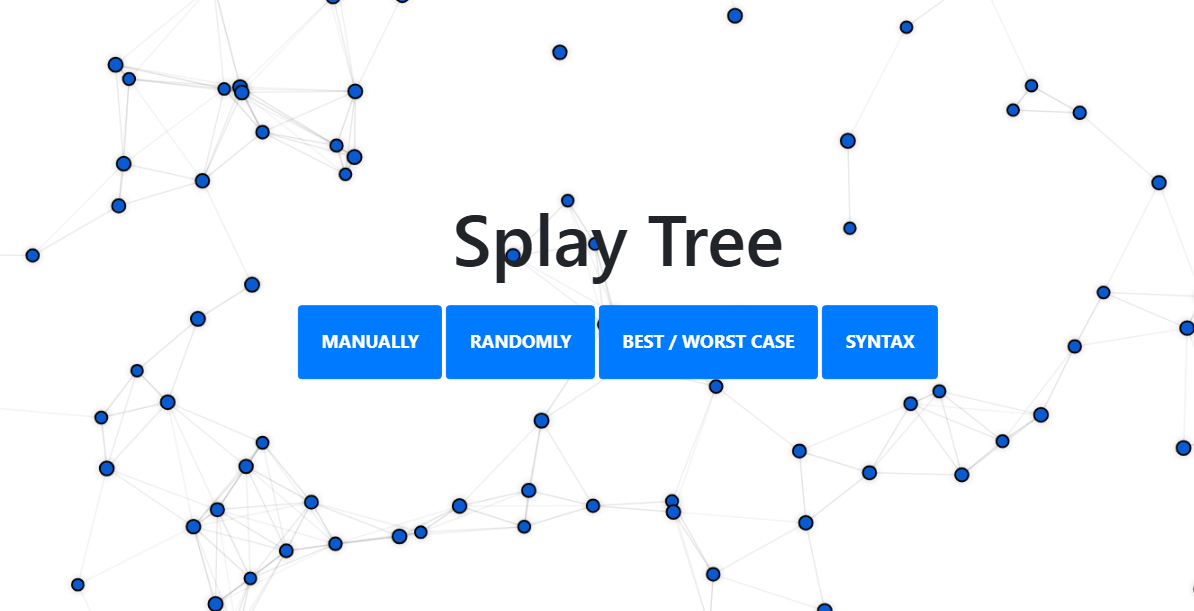
\includegraphics[width=0.9\textwidth]{Figures/input_modes_menu.png}
    \caption{Hlavní nabídka režimů zadávání vstupů u zvoleného algoritmu}
    \label{fig:input_modes_menu}
\end{figure}

Na obrázku \ref{fig:input_modes_menu} je znázorněna hlavní nabídka režimů zadávání vstupů, která je uživateli k dispozici po zvolení konkrétního algoritmu. Obrázek \ref{fig:input_modes_examples} pak ukazuje konkrétní podobu jednotlivých režimů zadávání, konkrétně ruční zadávání vstupů, náhodné generování, výběr nejlepšího nebo nejhoršího případu a zadávání vstupů pomocí syntaxe příkazů.

\begin{figure}[!h]
    \centering
    \subfloat[Ruční zadávání vstupů]{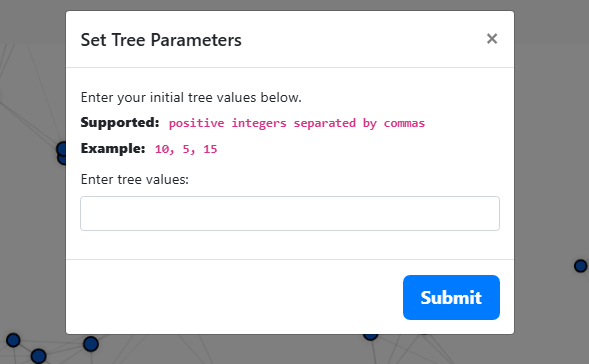
\includegraphics[width=0.45\textwidth]{Figures/input_manual.png}}
    \hfill
    \subfloat[Náhodné generování vstupů]{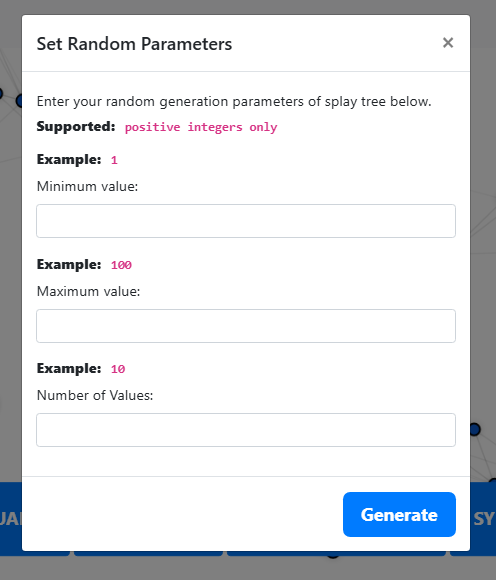
\includegraphics[width=0.45\textwidth]{Figures/input_random.png}} \\[0.5em]
    \subfloat[Volba nejlepšího/nejhoršího případu]{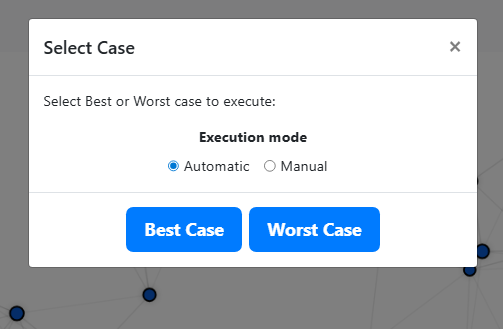
\includegraphics[width=0.45\textwidth]{Figures/input_bestworst.png}}
    \hfill
    \subfloat[Zadávání vstupů pomocí syntaxe příkazů]{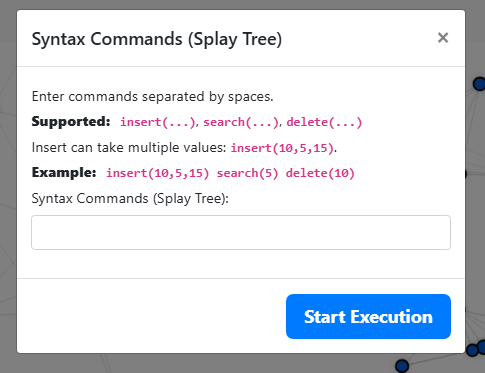
\includegraphics[width=0.45\textwidth]{Figures/input_syntax.png}}
    \caption{Příklady jednotlivých režimů zadávání vstupů}
    \label{fig:input_modes_examples}
\end{figure}

\newpage

\subsection{Zobrazení průběhu algoritmu po jednotlivých krocích}
Další důležitou součástí návrhu funkcionality komponenty bylo zobrazení průběhu algoritmu po jednotlivých krocích. Pro výuku amortizované složitosti totiž nestačí uživateli ukázat pouze konečný výsledek, ale je nutné umožnit mu sledovat, co se děje v průběhu celého výpočtu. Komponenta proto byla navržena tak, aby uživatel mohl vidět postupný vývoj algoritmu a změny stavu datové struktury v jednotlivých krocích simulace.

Takové zobrazení je důležité především proto, že studentovi umožňuje lépe pochopit návaznost jednotlivých operací a jejich vliv na další chování algoritmu. Díky krokovému průběhu lze sledovat nejen samotný výsledek operace, ale i způsob, jakým k němu algoritmus dospívá. Návrh této funkcionality proto představuje jednu z klíčových částí celé komponenty.

Na obrázku \ref{fig:syntax_step_mode} je znázorněn průběh algoritmu v režimu syntaxe, kde uživatel postupuje jednotlivými kroky simulace a může sledovat aktuální stav datové struktury i informace o právě prováděné operaci. Obrázek \ref{fig:bestworst_auto_mode} pak ukazuje automatický průběh v režimu nejlepšího/nejhoršího případu, kde se předem připravený scénář vykonává postupně bez nutnosti ručního zadávání každého kroku.

\begin{figure}[H]
    \centering
    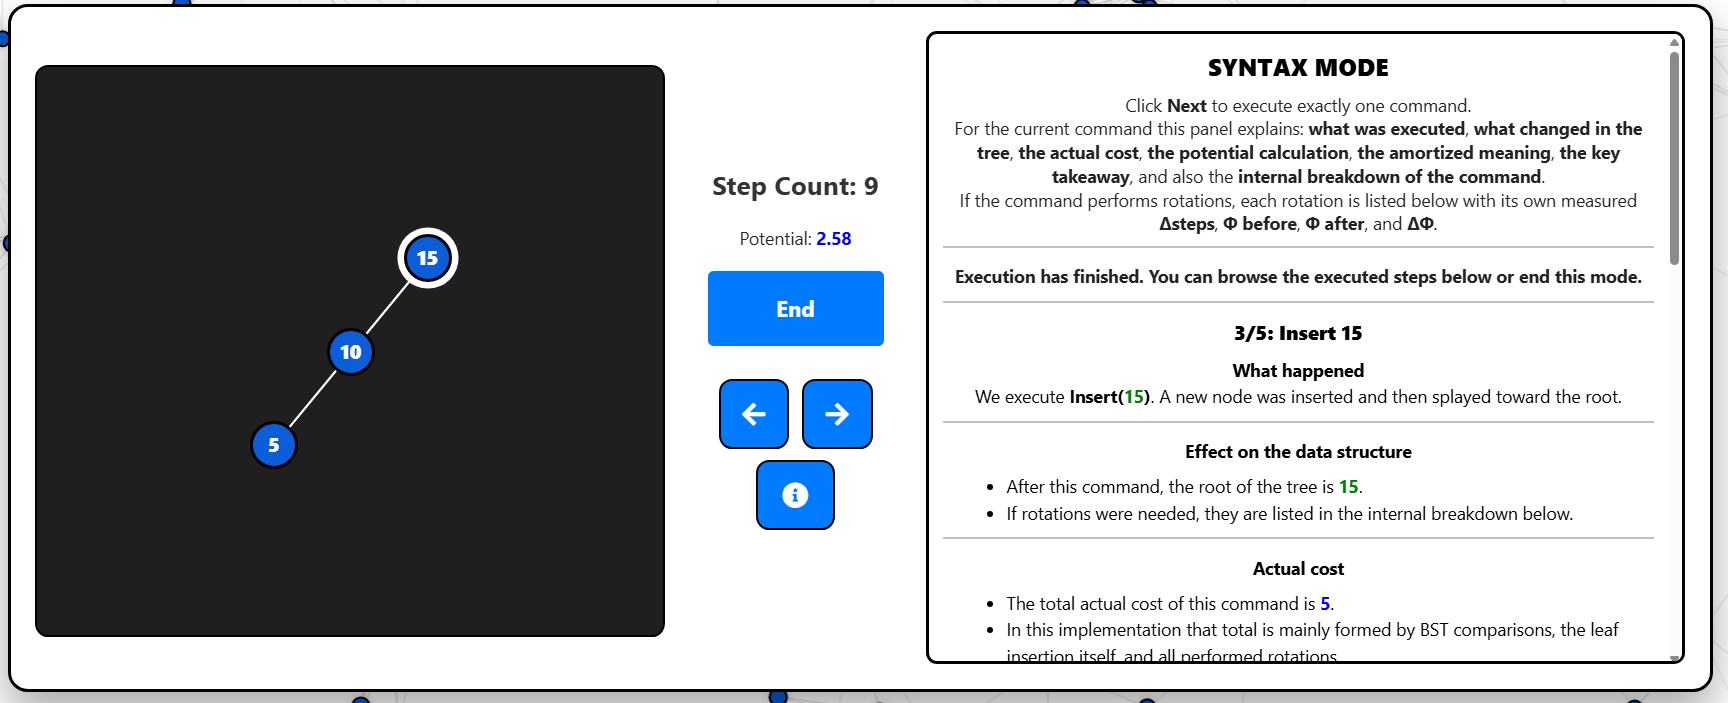
\includegraphics[width=0.95\textwidth]{Figures/syntax_step_mode.png}
    \caption{Zobrazení průběhu algoritmu po jednotlivých krocích v režimu syntaxe}
    \label{fig:syntax_step_mode}
\end{figure}

\begin{figure}[H]
    \centering
    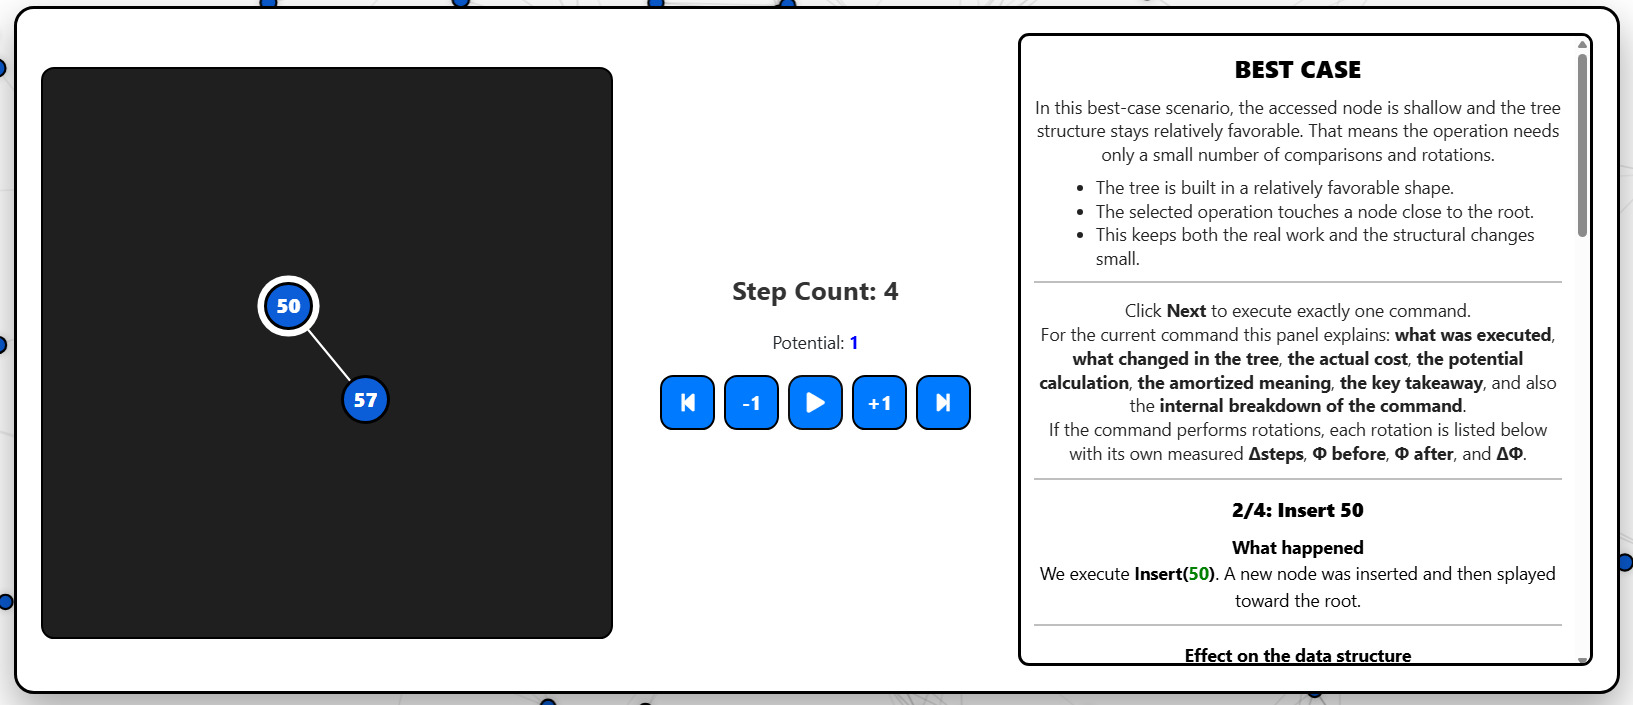
\includegraphics[width=0.95\textwidth]{Figures/bestworst_auto_mode.png}
    \caption{Automatický průběh simulace v režimu nejlepšího/nejhoršího případu}
    \label{fig:bestworst_auto_mode}
\end{figure}

\newpage

\subsection{Zobrazení počtu kroků a potenciálu}
Pro správné pochopení amortizované analýzy bylo při návrhu důležité zohlednit také zobrazení hodnot, které s tímto typem hodnocení přímo souvisejí. Komponenta proto měla zobrazovat počet provedených kroků a zároveň i hodnotu potenciálu, případně jinou odpovídající veličinu podle použité metody analýzy. Tyto hodnoty nemají sloužit pouze jako doplněk vizualizace, ale jako důležitá součást výkladu toho, proč se chování algoritmu hodnotí určitým způsobem.

Zobrazení počtu kroků a potenciálu umožňuje uživateli sledovat nejen to, co algoritmus právě vykonává, ale také to, jak se mění hodnoty důležité pro celkovou interpretaci jeho amortizované složitosti. Student tak může lépe pochopit vztah mezi jednotlivými operacemi, jejich skutečnými náklady a dlouhodobým chováním algoritmu v rámci celé posloupnosti operací.

Na obrázku \ref{fig:step_count_potential} je ukázáno zobrazení počtu provedených kroků a aktuální hodnoty potenciálu v průběhu simulace. Tyto informace jsou součástí hlavního rozhraní komponenty a tvoří důležitou oporu při sledování vývoje algoritmu i při interpretaci jeho amortizované složitosti.

\begin{figure}[H]
    \centering
    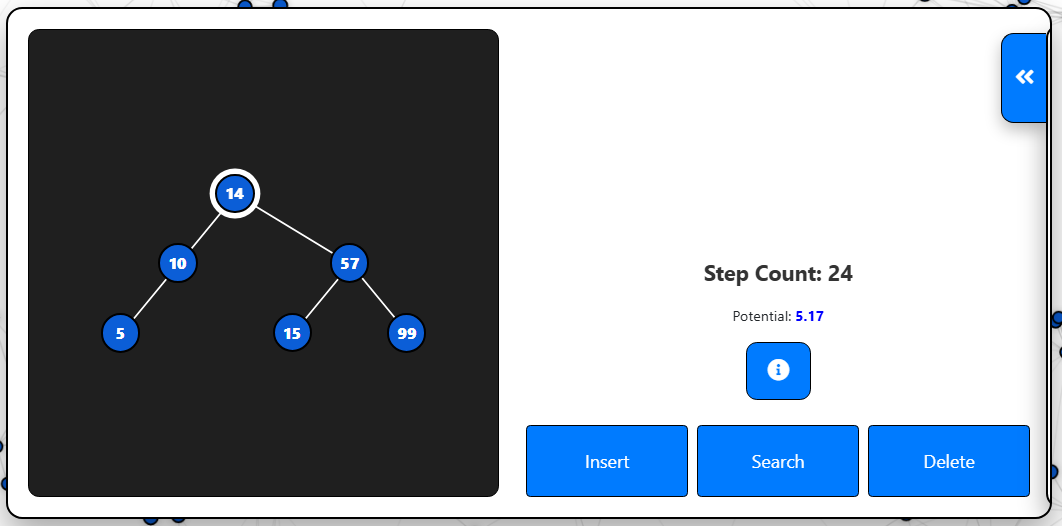
\includegraphics[width=0.95\textwidth]{Figures/step_count_potential.png}
    \caption{Zobrazení počtu kroků a aktuální hodnoty potenciálu v průběhu simulace}
    \label{fig:step_count_potential}
\end{figure}

\newpage

\subsection{Zobrazení doplňujících informací o aktuálním stavu algoritmu}
Součástí návrhu funkcionality komponenty bylo také zobrazení doplňujících informací o aktuálním stavu algoritmu. Samotná vizualizace datové struktury nebo zobrazení provedené operace totiž nemusí být vždy dostačující k tomu, aby uživatel přesně porozuměl tomu, co se v daném okamžiku děje. Z tohoto důvodu bylo vhodné doplnit průběh simulace o textové a přehledně uspořádané informace, které uživateli usnadní orientaci.

Tyto doplňující informace mají pomoci objasnit význam aktuálního kroku, stav datové struktury nebo souvislosti mezi právě prováděnou operací a chováním algoritmu jako celku. Uživatel tak nemá k dispozici pouze vizuální podobu aktuálního stavu, ale také slovní vysvětlení toho, co bylo provedeno, co se změnilo a jaký dopad má daný krok z hlediska amortizované analýzy. Návrh této části funkcionality tak podporuje srozumitelnost komponenty a přispívá k tomu, aby uživatel mohl lépe propojit vizuální průběh simulace s teoretickým výkladem algoritmu.

Na obrázku \ref{fig:history_info_panel} je znázorněn příklad detailních informací dostupných v historii vykonaných kroků. Obrázek \ref{fig:manual_info_panel} pak ukazuje doplňující informační panel přímo v průběhu práce s algoritmem, kde jsou zobrazeny informace vztahující se k aktuálně prováděné operaci.

\begin{figure}[H]
    \centering
    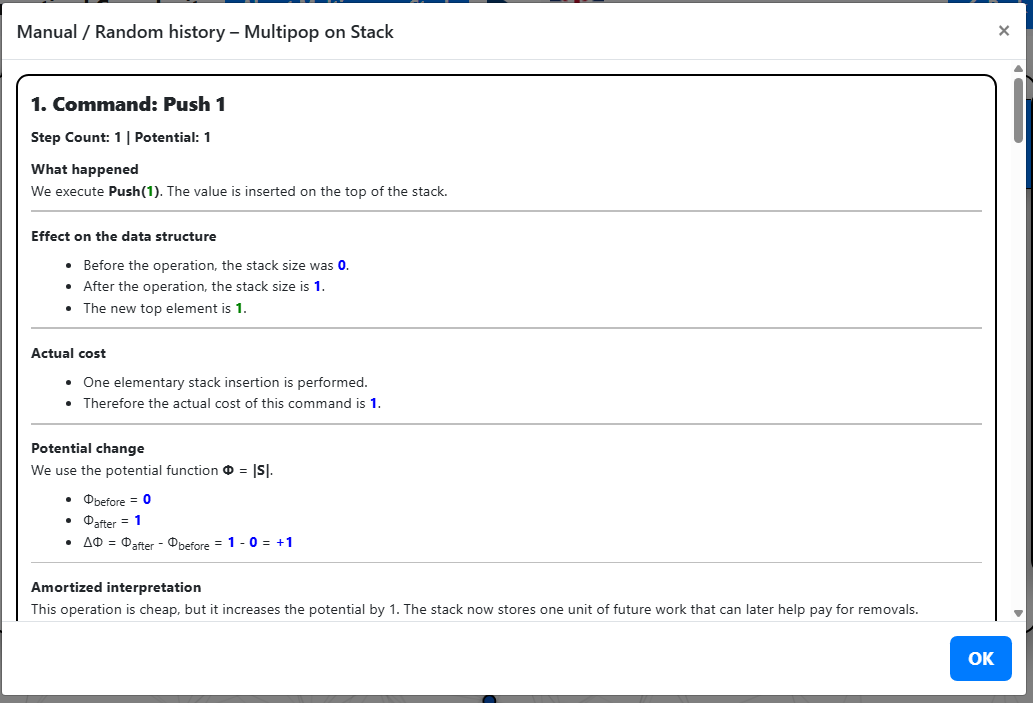
\includegraphics[width=0.92\textwidth]{Figures/history_info_panel.png}
    \caption{Detailní doplňující informace dostupné v historii provedených kroků}
    \label{fig:history_info_panel}
\end{figure}

\begin{figure}[H]
    \centering
    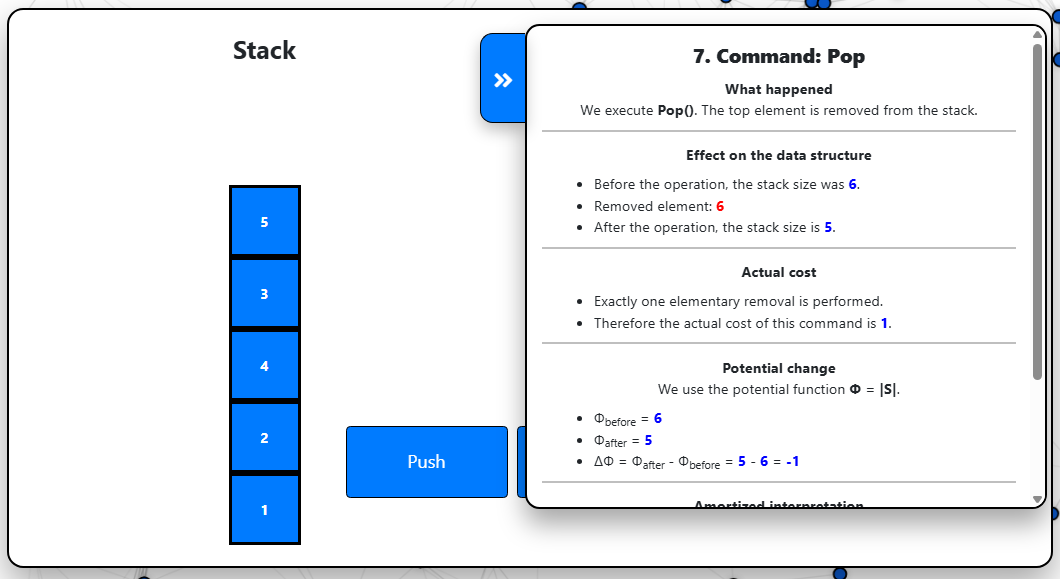
\includegraphics[width=0.92\textwidth]{Figures/manual_info_panel.png}
    \caption{Doplňující informační panel zobrazující aktuální stav operace při práci s algoritmem}
    \label{fig:manual_info_panel}
\end{figure}



\section{Návrh uživatelského rozhraní}
V této části je popsán návrh UI navrhované komponenty. Nejprve je pozornost věnována návrhu hlavní stránky a způsobu výběru jednotlivých algoritmů. Následně jsou shrnuty základní ovládací prvky simulace a způsob vizualizace použitých datových struktur. V závěru této části je popsán návrh informačních panelů a doprovodných vysvětlení, která mají podpořit výukový charakter komponenty.

\subsection{Návrh hlavní stránky a výběru algoritmu}
Při návrhu uživatelského rozhraní bylo důležité vytvořit hlavní stránku, která bude pro uživatele přehledná a umožní mu rychlou orientaci v celé komponentě. Hlavní stránka proto byla navržena jako výchozí rozcestník, z něhož si uživatel vybírá konkrétní algoritmus, se kterým chce dále pracovat. Současně bylo cílem, aby již na této úrovni bylo zřejmé, že komponenta slouží jako součást výukového prostředí zaměřeného na amortizovanou složitost.

Velký důraz byl kladen na jednoduchost výběru jednotlivých algoritmů. Uživatel má mít možnost z hlavní stránky přímo přejít k vybranému algoritmu, aniž by musel procházet složitější strukturu nabídek. Návrh proto počítal s výrazným zobrazením všech tří algoritmů zařazených do praktické části práce. Tím je zajištěno, že uživatel ihned vidí, jaké algoritmy jsou v komponentě dostupné, a může si zvolit ten, který chce právě vyzkoušet.

Součástí návrhu hlavní stránky byly také další prvky podporující orientaci a dostupnost informací. Patří mezi ně zejména možnost přepínání jazykových preferencí a přístup k doplňujícím informacím o samotné bakalářské práci. Hlavní stránka tak neslouží pouze jako technický vstup do aplikace, ale zároveň plní orientační a informační funkci.

Na obrázku \ref{fig:main_page_algorithm_selection} je znázorněna hlavní stránka komponenty, na níž jsou zobrazeny dostupné algoritmy, přepínač jazykových preferencí a tlačítko pro zobrazení informací o bakalářské práci.

\begin{figure}[H]
    \centering
    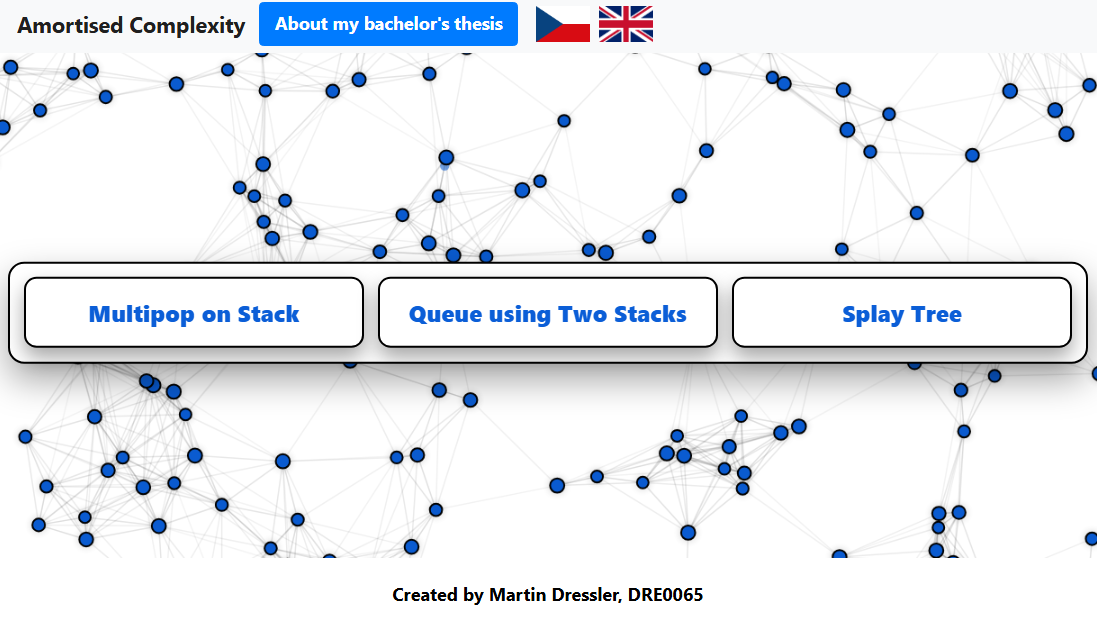
\includegraphics[width=0.95\textwidth]{Figures/main_page_algorithm_selection.png}
    \caption{Hlavní stránka komponenty s výběrem algoritmů, přepínačem jazykových mutací a tlačítkem pro informace o bakalářské práci}
    \label{fig:main_page_algorithm_selection}
\end{figure}

\subsection{Návrh ovládacích prvků simulace}
Součástí návrhu uživatelského rozhraní bylo také vytvoření vhodných ovládacích prvků simulace. Tyto prvky musely uživateli umožnit pohodlně řídit průběh algoritmu a současně podporovat srozumitelné sledování jednotlivých kroků. Návrh proto počítal s tím, že uživatel nebude pouze pasivně sledovat vykonávání algoritmu, ale bude moci průběh simulace aktivně ovlivňovat.

Důležitou součástí ovládání bylo zejména krokování mezi jednotlivými stavy simulace. Uživatel má mít možnost přecházet na předchozí nebo následující krok, ukončit aktuální režim a podle potřeby si zobrazit také doplňující historii informací. Ovládací prvky proto byly navrženy tak, aby byly snadno dostupné a přehledně oddělené od samotné vizualizace datové struktury. Tím je zajištěno, že uživatel může současně sledovat stav algoritmu i pohodlně pracovat s jeho ovládáním.

Na obrázku \ref{fig:simulation_controls} je znázorněn příklad návrhu ovládacích prvků simulace v režimu syntaxe. Součástí rozhraní jsou tlačítka pro pohyb mezi jednotlivými kroky, tlačítko pro ukončení režimu a tlačítko pro zobrazení historie informací.

\begin{figure}[H]
    \centering
    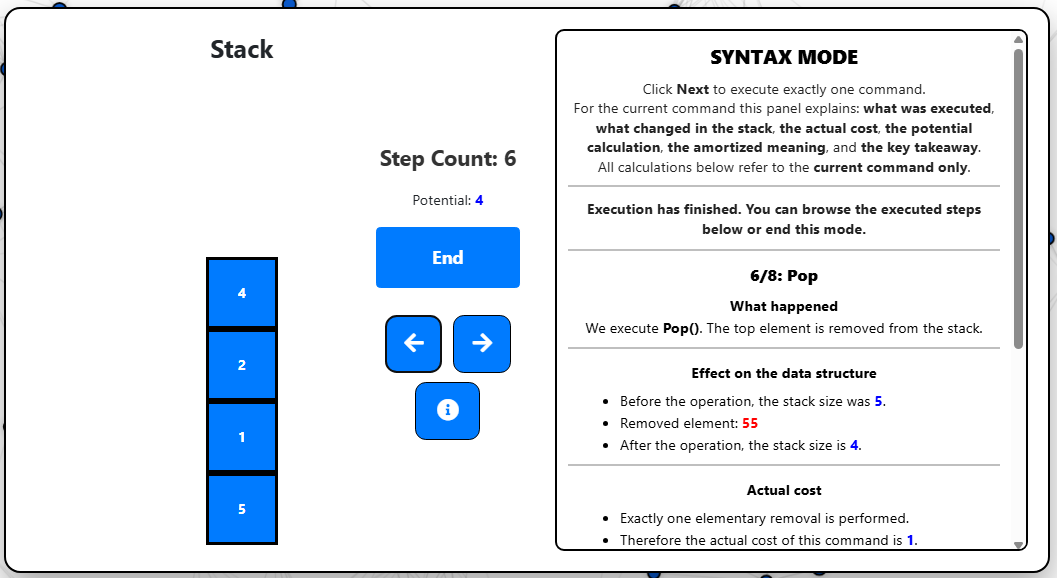
\includegraphics[width=0.95\textwidth]{Figures/simulation_controls.png}
    \caption{Příklad ovládacích prvků simulace v režimu syntaxe}
    \label{fig:simulation_controls}
\end{figure}

\subsection{Návrh vizualizace datových struktur}
Důležitou součástí návrhu uživatelského rozhraní bylo také zobrazení datových struktur používaných jednotlivými algoritmy. Cílem nebylo pouze zobrazit stav výpočtu formou číselných hodnot, ale navrhnout takovou vizualizaci, která uživateli umožní co nejlépe pochopit změny struktury v průběhu simulace. Z tohoto důvodu byla podoba vizualizace přizpůsobena konkrétnímu typu datové struktury, s níž daný algoritmus pracuje.

U algoritmu Multipop na zásobníku byla zvolena jednoduchá svislá reprezentace zásobníku, která přehledně ukazuje pořadí prvků i změny na vrcholu zásobníku. U fronty využívající dva zásobníky bylo naopak důležité oddělit oba zásobníky tak, aby bylo zřejmé, do které části se prvky vkládají a ze které se odebírají. U Splay stromu pak bylo nezbytné navrhnout stromovou vizualizaci, která umožní sledovat nejen obsah uzlů, ale i jejich vzájemné propojení a změny struktury při jednotlivých operacích.

Takto navržená vizualizace datových struktur podporuje názornost celé komponenty a umožňuje uživateli lépe porozumět tomu, jak se algoritmus chová při různých operacích. Uživatel tak nesleduje pouze výsledky výpočtu, ale i konkrétní změny uspořádání dat, které jsou pro pochopení amortizované složitosti důležité.

Na obrázku \ref{fig:data_structure_visualizations} jsou znázorněny příklady vizualizace datových struktur použitých v jednotlivých algoritmech, konkrétně zásobníku, fronty realizované pomocí dvou zásobníků a Splay stromu.

\begin{figure}[H]
    \centering
    \subfloat[Zásobník]{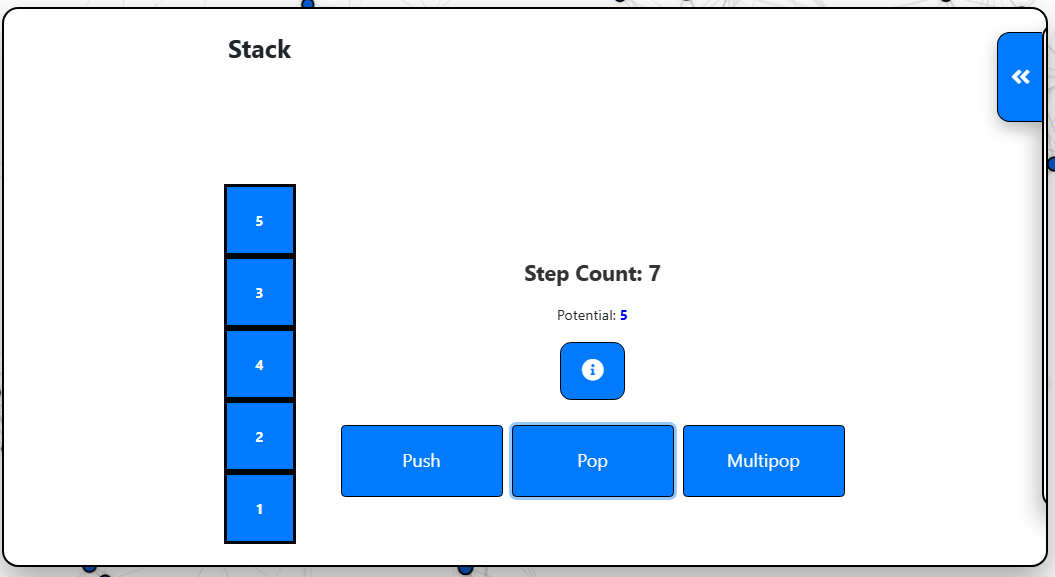
\includegraphics[width=0.6\textwidth]{Figures/stack_visualization.png}}
    \hfill
    \subfloat[Fronta využívající dva zásobníky]{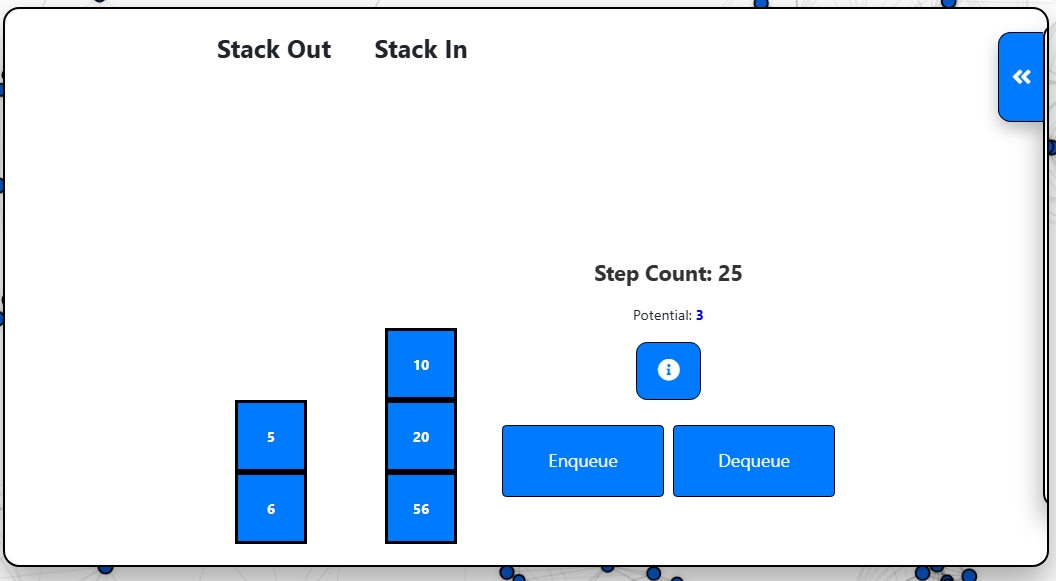
\includegraphics[width=0.6\textwidth]{Figures/queue_visualization.png}}
    \hfill
    \subfloat[Splay strom]{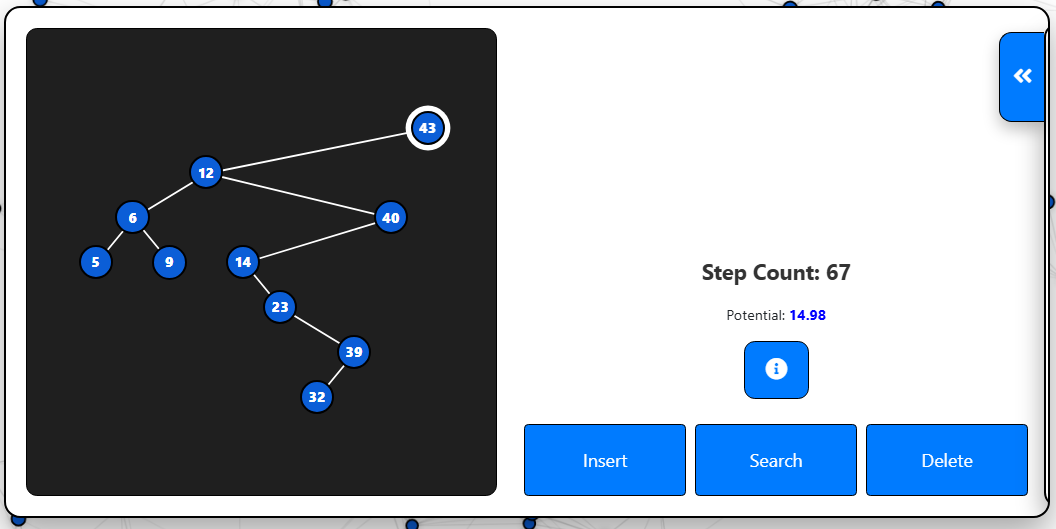
\includegraphics[width=0.6\textwidth]{Figures/splay_visualization.png}}
    \caption{Příklady vizualizace datových struktur použitých v navrhované komponentě}
    \label{fig:data_structure_visualizations}
\end{figure}

\subsection{Návrh informačních panelů a doprovodných vysvětlení o algoritmech}
Součástí návrhu uživatelského rozhraní byly také informační panely a doprovodná vysvětlení vztahující se k jednotlivým algoritmům. Cílem těchto částí rozhraní nebylo pouze doplnit simulaci o další text, ale nabídnout uživateli přehledné vysvětlení základních vlastností algoritmu, použitých operací a jeho vztahu k amortizované analýze. Díky tomu může uživatel získat potřebný teoretický kontext ještě před samotnou prací se simulací nebo v jejím průběhu.

Návrh těchto informačních panelů vycházel z potřeby propojit praktickou ukázku s doprovodným výkladem. Uživatel tak nemá k dispozici pouze vizualizaci datové struktury a ovládací prvky simulace, ale také souvislý popis algoritmu, jeho hlavní myšlenky a vysvětlení, proč je daný algoritmus vhodný pro amortizovanou analýzu. Takové řešení podporuje lepší orientaci v problematice a současně posiluje výukový charakter celé komponenty.

Na obrázku \ref{fig:algorithm_info_panel} je znázorněn příklad informačního panelu věnovaného jednomu z vybraných algoritmů. Panel obsahuje základní popis algoritmu, přehled jeho operací, hlavní princip fungování i stručné vysvětlení jeho složitosti z hlediska amortizované analýzy.

\begin{figure}[H]
    \centering
    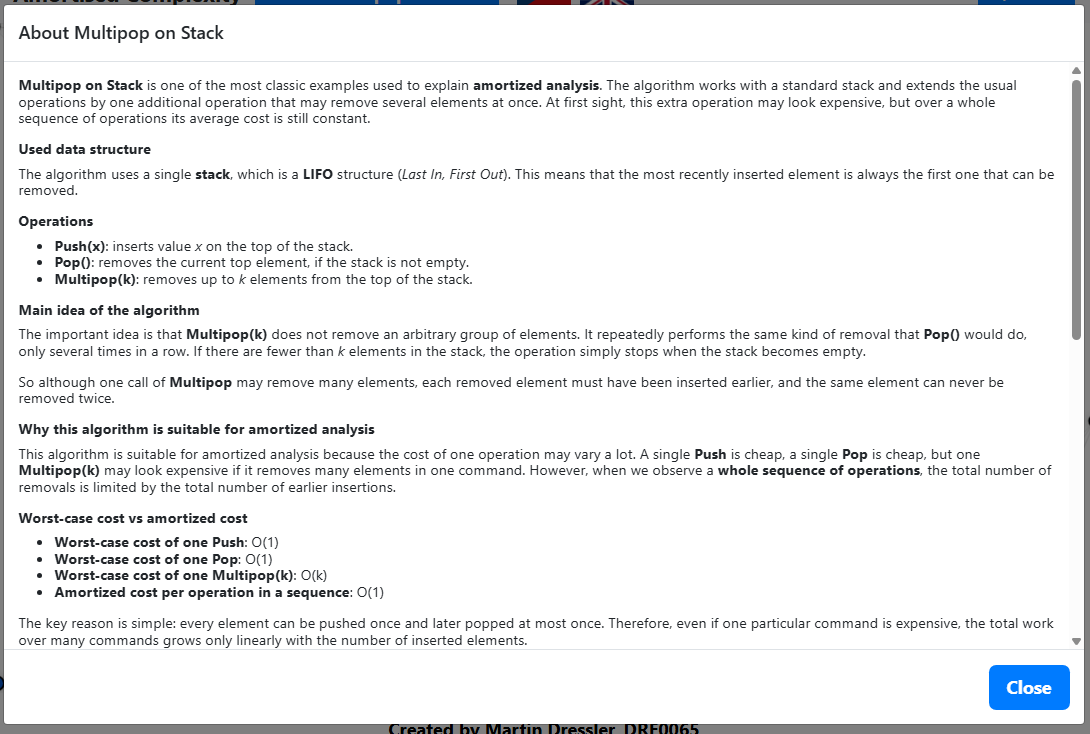
\includegraphics[width=0.95\textwidth]{Figures/algorithm_info_panel.png}
    \caption{Příklad informačního panelu s doprovodným vysvětlením vybraného algoritmu}
    \label{fig:algorithm_info_panel}
\end{figure}



\section{Návrh struktury komponenty}
Tato část se zaměřuje na návrh celkové struktury komponenty a na rozdělení jejích jednotlivých částí. Nejprve je popsáno oddělení společných prvků od částí specifických pro jednotlivé algoritmy. Následně je objasněna návaznost jednotlivých částí komponenty při práci uživatele. V závěru je pozornost věnována také možnostem budoucího rozšíření navrženého řešení.

\subsection{Rozdělení komponenty na společnou a algoritmicky specifickou část}
Celá struktura komponenty je rozdělena na prvky, které jsou společné pro všechny algoritmy, a na prvky, které jsou vytvořeny přímo pro konkrétní algoritmus. Mezi prvky patřící do společné části tvoří zejména hlavní stránka, výběr algoritmů, rozložení UI, obecné ovládací prvky a některé informační panely. Naopak část specifická pro daný algoritmus zahrnuje například samotnou logiku jednotlivých algoritmů, jejich konkrétní operace, způsob vizualizace příslušné datové struktury a doprovodné informace vztahující se k danému algoritmu. Díky tomuto rozdělení je možné zachovat jednotný vzhled a princip ovládání celé komponenty, ale zároveň ponechat dostatečný prostor pro přizpůsobení jednotlivým algoritmům.

\subsection{Návaznost jednotlivých částí komponenty}
Při návrhu byl brán zřetel také na návaznost jednotlivých částí z pohledu uživatele. Práce s komponentou začíná na hlavní stránce, kde si uživatel zvolí konkrétní algoritmus. Poté si vybere typ vstupu a sleduje průběh algoritmu, hodnoty důležité pro amortizovanou analýzu a doplňující vysvětlení. Jednotlivé části komponenty byly vytvořeny tak, aby na sebe logicky navazovaly a vytvářely ucelené prostředí pro práci uživatele.

\subsection{Možnosti budoucího rozšíření}
Při návrhu struktury bylo vhodné zohlednit také možnost budoucího rozšíření. Pokud by bylo potřeba aplikaci v budoucnu dále rozšířit, neměl by být problém přidat další algoritmy vhodné pro amortizovanou analýzu, aniž by bylo nutné zásadně měnit základní princip fungování celé komponenty. Stejným způsobem by bylo možné rozšiřovat informační panely, přidávat nové režimy práce se vstupy a další prvky.